%\title{Presentation Template}
\documentclass[10pt]{beamer}

\usetheme[progressbar=frametitle]{metropolis}
\usepackage{appendixnumberbeamer}

\usepackage[compatibility=false]{caption}
\usepackage{subcaption}
\usepackage{csquotes}
\usepackage{booktabs}
\usepackage{hyperref}
\usepackage[scale=2]{ccicons}
\usepackage{tikz}
\usepackage{bm}

\usepackage{multimedia}
\usepackage{media9}

\graphicspath{{./img/}}

\usepackage{pgfplots}
\usepgfplotslibrary{dateplot}

\usepackage{xspace}
\newcommand{\themename}{\textbf{\textsc{metropolis}}\xspace}

\title{Space-Filling Trees for Scalable Spatial Computing}
%\subditle{}
%\date{}
\author{Matthew Andres Moreno \newline \texttt{mmore500@msu.edu}}
\titlegraphic{\hfill\includegraphics[height=2cm]{img/MSU-Wordmark-Black}}

\begin{document}

\maketitle

% \begin{frame}{Table of contents}
%   \setbeamertemplate{section in toc}[sections numbered]
%   \tableofcontents[hideallsubsections]
% \end{frame}

% \section{Section}

\begin{frame}{Problem}

\begin{columns}
\begin{column}{0.225\textwidth}
\raggedleft
\Huge
N
\end{column}
\begin{column}{0.65\textwidth}
\centering

\includegraphics[width=\textwidth]{htree/grid}
\end{column}
\begin{column}{0.225\textwidth}
\end{column}
\end{columns}

\begin{columns}
\begin{column}{0.225\textwidth}
\end{column}
\begin{column}{0.65\textwidth}
\centering
\Huge
N
\end{column}
\begin{column}{0.225\textwidth}
\end{column}
\end{columns}

\end{frame}

\begin{frame}{Problem}

\begin{columns}
\begin{column}{0.225\textwidth}
\raggedleft
\Huge
N
\end{column}
\begin{column}{0.65\textwidth}
\centering
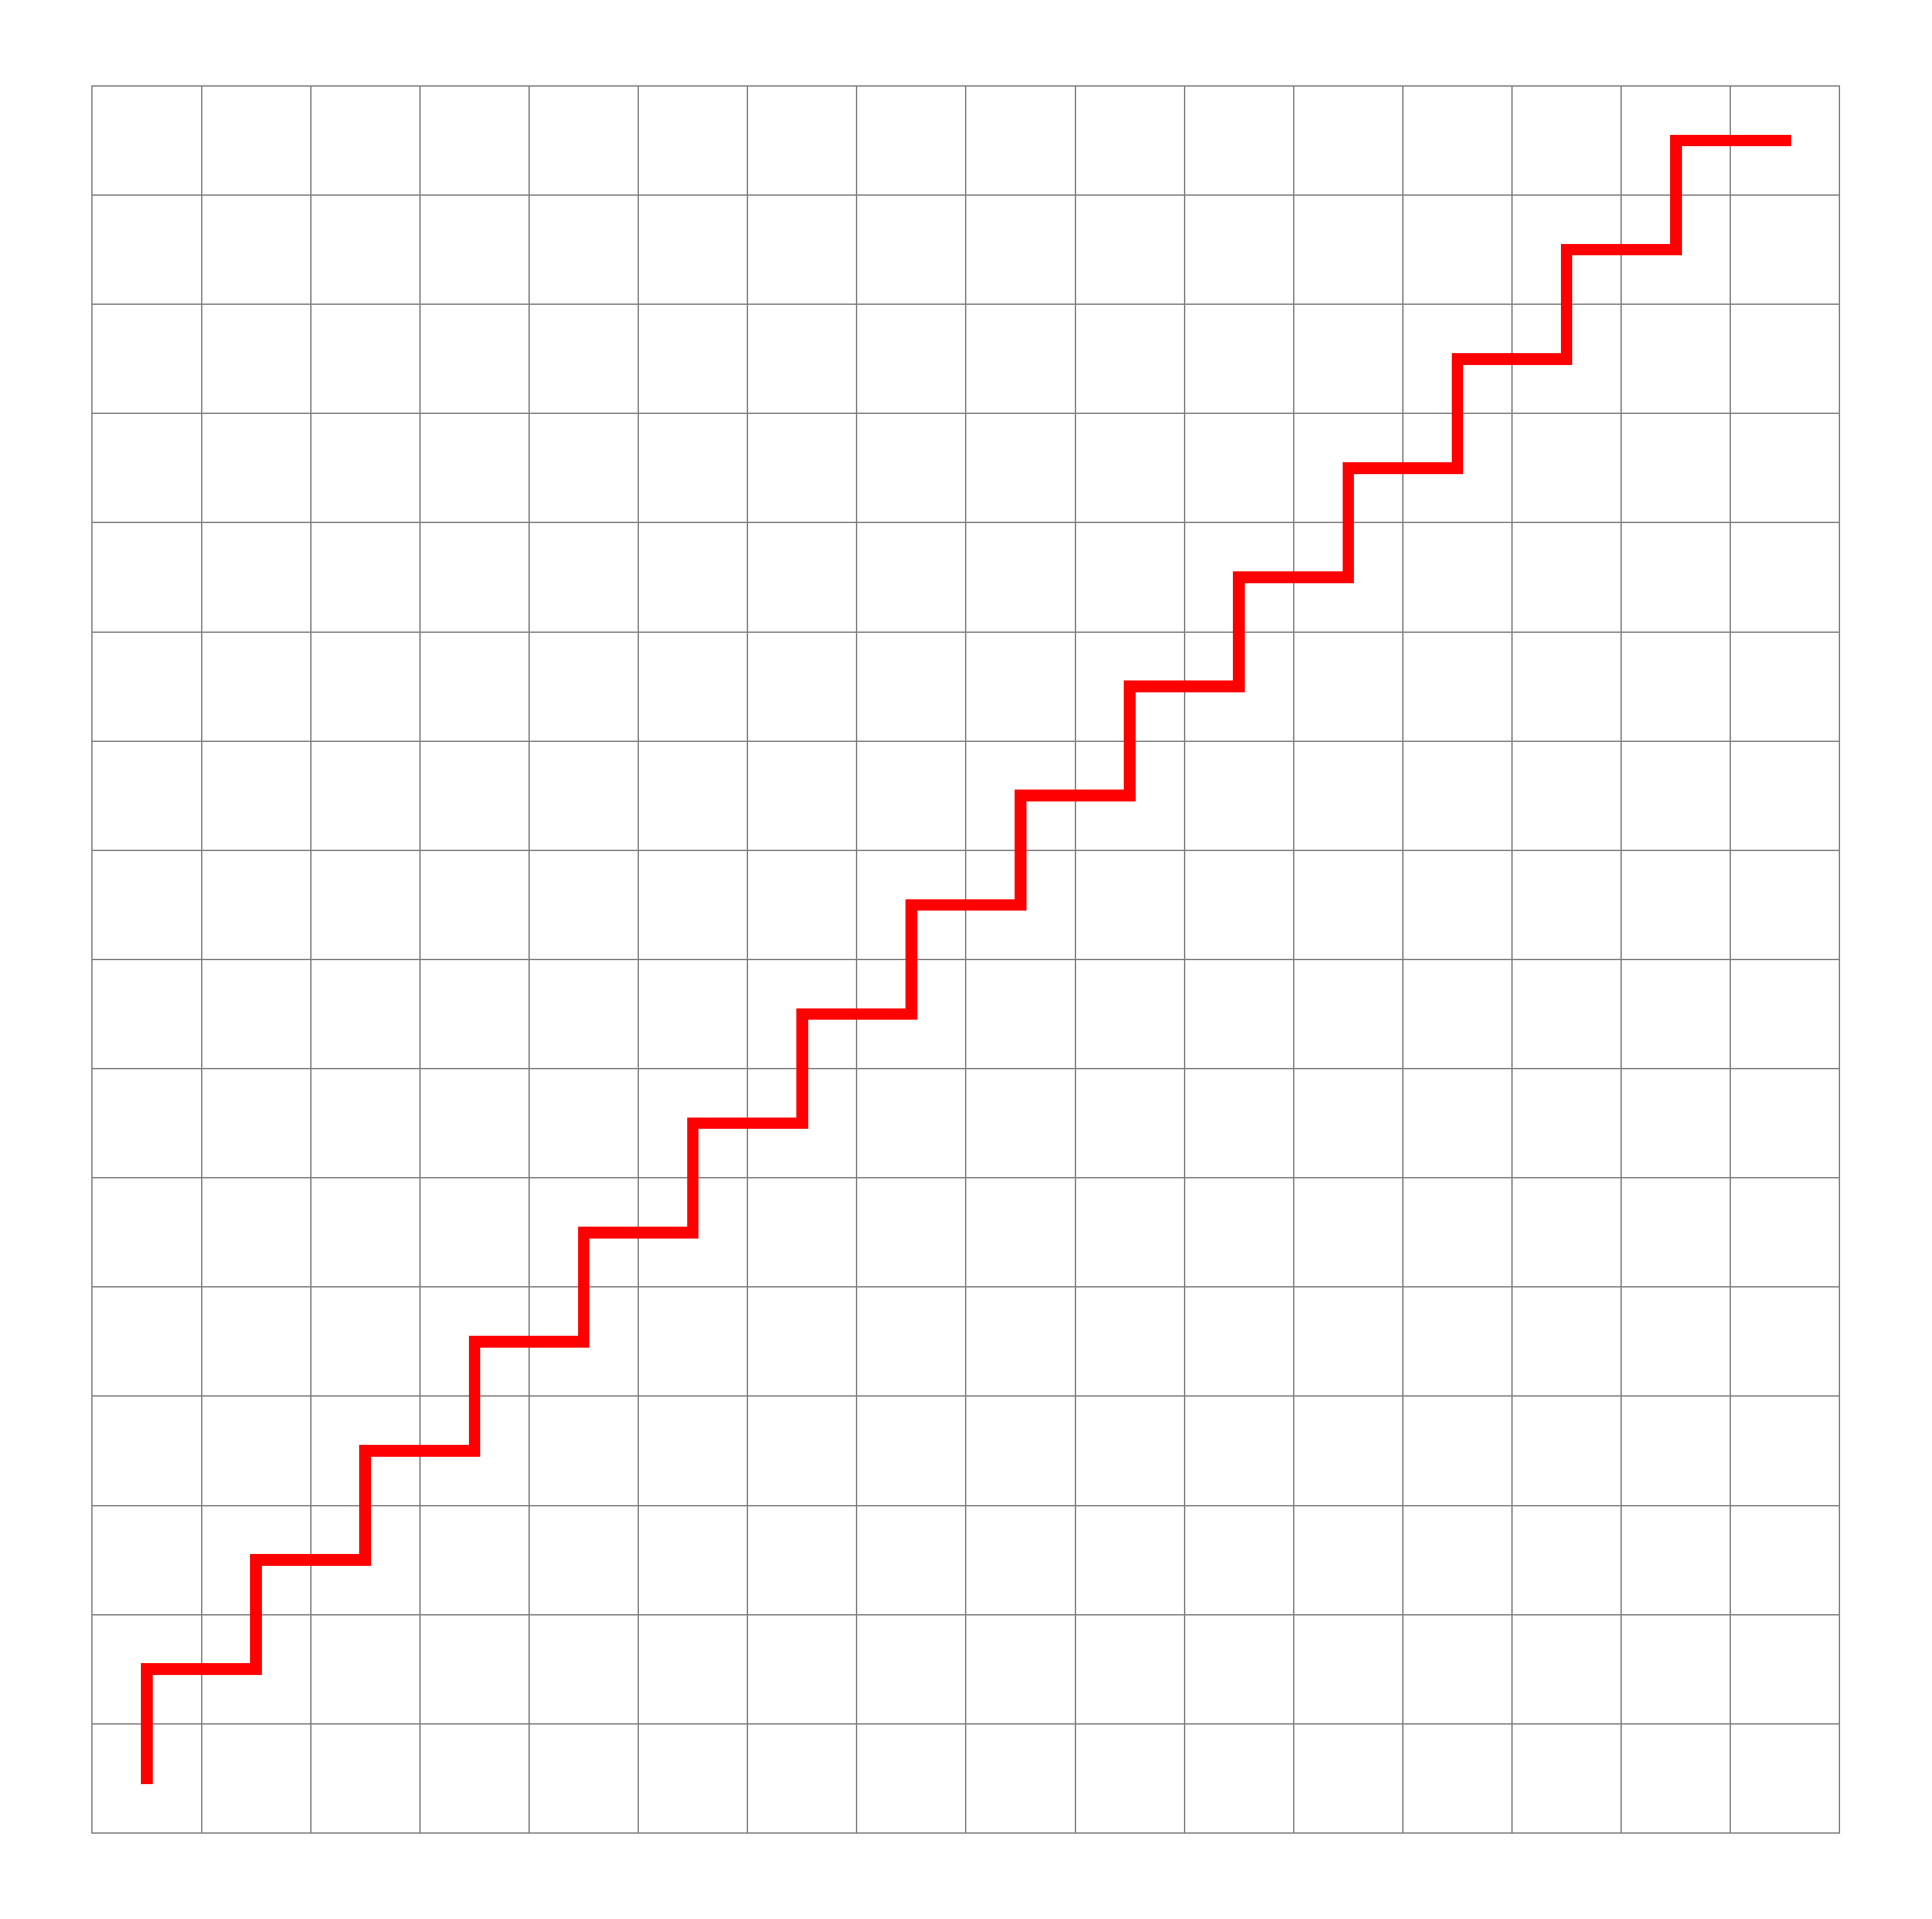
\includegraphics[width=\textwidth]{htree/grid-small-zigzag}
\end{column}
\begin{column}{0.225\textwidth}
\end{column}
\end{columns}

\begin{columns}
\begin{column}{0.225\textwidth}
\end{column}
\begin{column}{0.65\textwidth}
\centering
\Huge
N
\end{column}
\begin{column}{0.225\textwidth}
\end{column}
\end{columns}

\end{frame}

\begin{frame}{Problem}

\begin{columns}
\begin{column}{0.225\textwidth}
\raggedleft
\Huge
N
\end{column}
\begin{column}{0.65\textwidth}
\centering
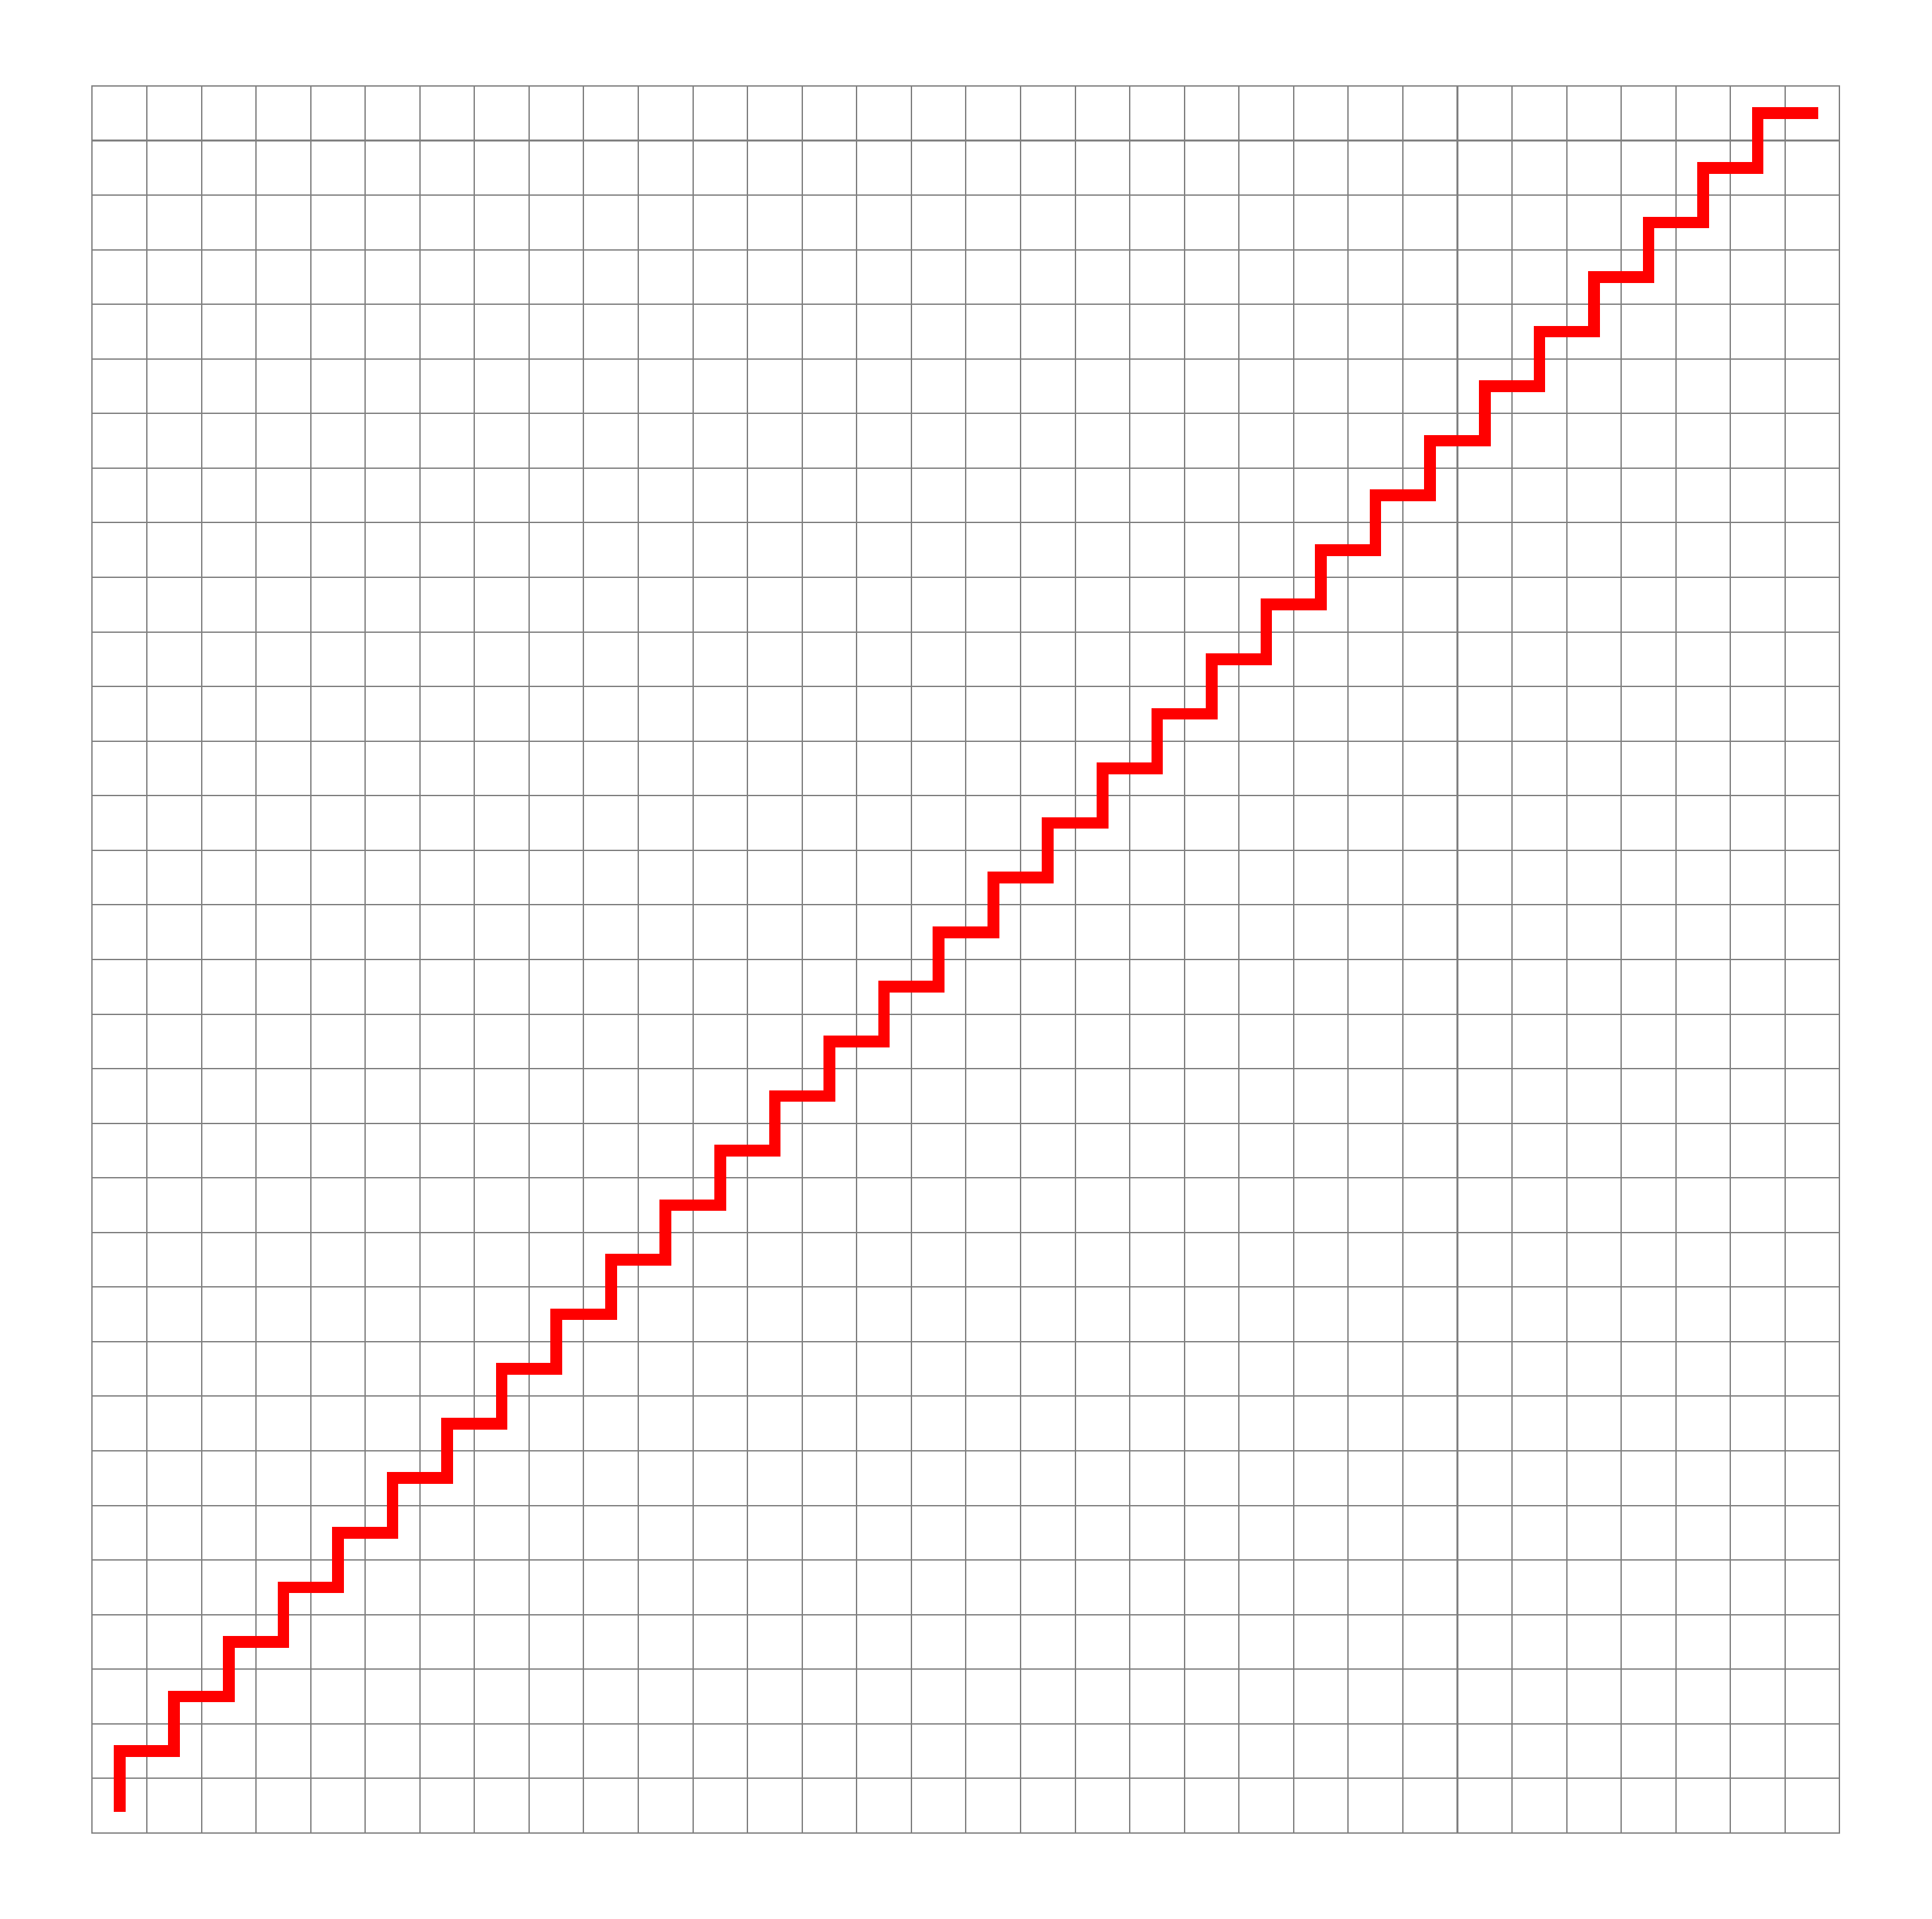
\includegraphics[width=\textwidth]{htree/grid-large-zigzag}
\end{column}
\begin{column}{0.225\textwidth}
\end{column}
\end{columns}

\begin{columns}
\begin{column}{0.225\textwidth}
\end{column}
\begin{column}{0.65\textwidth}
\centering
\Huge
N
\end{column}
\begin{column}{0.225\textwidth}
\end{column}
\end{columns}

\end{frame}

\begin{frame}{Problem}

$r$ number routers handling a message

$d$ distance between sender and receiver

{\Huge
\[
r \propto d
\]}

\end{frame}

\begin{frame}{Problem}

$\hat{l}$ mean router load

$\hat{s}$ mean per-node message send rate

$\hat{r}$ mean number routers handling each message

{\Huge
\[
\hat{l} = \hat{s} \times \hat{r}
\]}

\end{frame}

\begin{frame}{Problem}

$\hat{l}$ mean router load

$\hat{s}$ mean per-node message send rate

$\hat{d}$ mean message distance

{\Huge
\[
\hat{l} \propto \hat{s} \times \hat{d}
\]}

\end{frame}

\begin{frame}{Problem}

$\hat{l}$ mean router load

$\hat{s}$ mean per-node message send rate

$\hat{d} = F(N)$ mean message distance
\begin{itemize}
\item bounded? unbounded?
\item small-world network?
\end{itemize}

{\Huge
\[
\hat{l} \propto \hat{s} \times F(N)
\]}

\end{frame}

\begin{frame}{Proposal}

\begin{itemize}
\item reduce mean number routers handling each message with passive bypasses
\item space-filling tree
\end{itemize}

\end{frame}

\begin{frame}{Proposal}

\begin{columns}
\begin{column}{0.225\textwidth}
\raggedleft
\Huge
N
\end{column}
\begin{column}{0.65\textwidth}
\centering
\includegraphics[width=\textwidth]<1>{htree/grid}
\includegraphics[width=\textwidth]<2>{htree/const-tree-grid}
\includegraphics[width=\textwidth]<3>{htree/grid-small-treewalk}
\includegraphics[width=\textwidth]<4>{htree/grid-large-treewalk}
\end{column}
\begin{column}{0.225\textwidth}
\end{column}
\end{columns}

\begin{columns}
\begin{column}{0.225\textwidth}
\end{column}
\begin{column}{0.65\textwidth}
\centering
\Huge
N
\end{column}
\begin{column}{0.225\textwidth}
\end{column}
\end{columns}

\end{frame}

\begin{frame}{Proposal}

$\hat{l}$ mean router load

$\hat{s}$ mean per-node message send rate

$\hat{d} = F(N)$ mean message distance
\begin{itemize}
\item bounded? unbounded?
\item small-world network?
\end{itemize}

{\Huge
\[
\hat{l} \propto \hat{s} \times \log{f(N)}
\]}

\end{frame}

\begin{frame}{Proposal}

$\hat{d} = F(N) = \int_1^N f_N(n) \, dn$ mean message distance

\begin{itemize}
\item bounded? unbounded?
\item small-world network?
\item exponential decay? $f(n) = e^{-\beta N}$ $\rightarrow$ $F(N)$ bounded
  \begin{itemize}
    \item with naive connectivity, message latency $\propto N$
    \item with sfbt connectivity, message latency $\propto \log(N)$ (assuming router latency $>>$ wiring latency)
    \item even load over sfbt tree?
  \end{itemize}
\item power law? $f(n) = N^{-\alpha}$ $\rightarrow$ $F(N)$ unbounded
  \begin{itemize}
    \item load on high-level connections increases (explodes?) with N
    \item address by beefing high-level connections? (lose total hardware modular uniformity)
    \item address by sending only halfway up the tree?
    \begin{itemize}
      \item bandwidth increases exponentially $\propto N$
      \item number router hops now polynomial $r \propto log(d) + d^{1/2}$
    \end{itemize}
  \end{itemize}
\end{itemize}

\end{frame}

\begin{frame}{Proposal}

\begin{columns}
\begin{column}{0.225\textwidth}
\raggedleft
\Huge
N
\end{column}
\begin{column}{0.65\textwidth}
\centering
\includegraphics[width=\textwidth]<1>{htree/var-tree-grid}
\includegraphics[width=\textwidth]<2>{htree/const-tree-compl-grid}
\includegraphics[width=\textwidth]<3>{htree/var-tree-compl-grid}
\end{column}
\begin{column}{0.225\textwidth}
\end{column}
\end{columns}

\begin{columns}
\begin{column}{0.225\textwidth}
\end{column}
\begin{column}{0.65\textwidth}
\centering
\Huge
N
\end{column}
\begin{column}{0.225\textwidth}
\end{column}
\end{columns}

\end{frame}


\begin{frame}{Thinking More Generally}

$h$ hierarchical level

$c$ cell count

{\Huge
\[
c \propto e^h
\]
}

\end{frame}

\begin{frame}{Thinking More Generally}

$g$ generation time

$c$ cell count

{\Large
\[
g \propto \sqrt{c} \propto \sqrt{e^h} = e^{h/2} \text{~~~~~\small(grid-filling growth)}
\]}
versus
{\Large
\[
g \propto \log{c} \propto h \text{~~~~~\small(exponential growth)}
\]
}

true exponential growth in toroidal grid framework?

also, consider selection time frame

\end{frame}

\begin{frame}[allowframebreaks=0.8,t]{Lots of Questions}
\begin{itemize}
\item comparison to GPU, kilobots, Intel Single-Chip Cloud Computer, Illuminato X Machina
\item relative compute vs communication/signaling load
\item hierarchical design for small-world network communication
  \begin{itemize}
  \item latency and load vs scale
  \item compare to other complex systems: internet, social networks, economies, brain, etc.
  \end{itemize}
\item spatial dimensionality (2D vs 3D grid)
\item micro-controller vs. micro-processor
\item router hardware/algorithm
  \begin{itemize}
  \item how to deal with moving batons
  \item sending batons locally vs thru hierarchical fractal network
  \end{itemize}
\item fractal hierarchical network
  \begin{itemize}
  \item "space-filling tree"
  \item "stochastic fractal"
  \item rapidly-exploring random tree (RRT)
  \item 2D "H-tree"
  \item 3D "Space-filling Binary Tree"
  \end{itemize}
\item true indefinite scalability vs. pseudo-indefinite scalability
\item consider effects of various levels of component failure on performance, how to adapt to component failure
\item guarantees as to spatial regularity (i.e., how far up the tree do two nodes at a certain distance have to go)
  \begin{itemize}
  \item O(n) [?] redundant linkages (i.e., all adjacent mth level nodes connected)
  \end{itemize}
\item scaling by irregular amounts (i.e., does it need to scale by powers of 2? does it need to scale as a perfect square? can it be rectangular? can it be ragged?)
  \begin{itemize}
  \item O(n) [?] redundant linkages (i.e., all adjacent mth level nodes connected)
\end{itemize}
\item monitoring/data collection
\item programming
\end{itemize}

\end{frame}


% \input{tex/appendix.tex}

% \input{tex/backup.tex}

\end{document}
